\section{ASP.NET Core}
ASP.NET Core is a web framework developed by Microsoft, for developing web applications in the .NET Core framework.
It uses the quite popular Model-View-Controller design pattern as a basis for the architecture of the applications developed in it.
\subsection{Model-View-Controller design pattern}
The Model-View-Controller pattern is an architectural pattern that splits the application into three basic components, the model, the view, and the controller. Originally meant for GUI development, the pattern has been adapted into web development, and is used by many of the frameworks in the space.\cite{gangoffour}

\begin{figure}[H]
\centering
	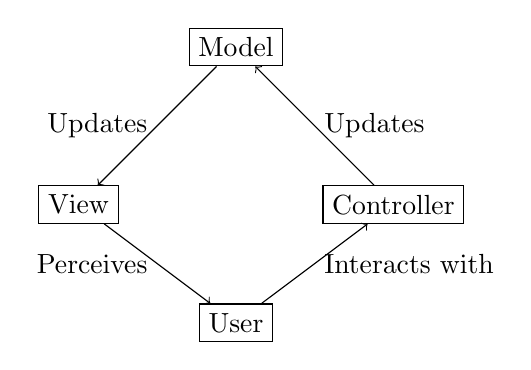
\begin{tikzpicture}[node distance=2cm]
	\node[draw] (model) {Model};
	\node[draw] (view) [below of=model, left of=model] {View};
	\node[draw] (controller) [below of=model, right of=model] {Controller};
	\draw[->] (model) -- node[left] {Updates} (view);
	\draw[->] (controller) -- node[right] {Updates} (model);
	\node[draw] (user) [below of=model, node distance=3.5cm] {User};
	\draw[->] (view) -- node[left] {Perceives} (user);
	\draw[->] (user) -- node[right] {Interacts with} (controller);
	\end{tikzpicture}
	\caption{The Model-View-Controller design pattern.}
\end{figure}

The basic idea of the pattern is that all of the data managed by the application is encapsulated into the model classes.
These can then be accessed or subscribed to by the views, which the user sees.
The user then subsequently interacts with the controller, which in turn updates the model.
The seperation of concerns allows for a quite flexible architecture, where you can change the view without touching the model or controller, or the controller without changing the view and model.\cite{gangoffour}
\subsection{Entity Framework}

